\documentclass{mproj}
\usepackage{graphicx}
\usepackage[backend=biber,
style=trad-abbrv]{biblatex}
\addbibresource{mproj.bib}
\usepackage{url}
\usepackage{fancyvrb}
\usepackage{float}
\usepackage[final]{pdfpages}
\usepackage{hyperref}
\hypersetup{
	urlcolor=blue}
\usepackage{fancyhdr}

% for alternative page numbering use the following package
% and see documentation for commands
%\usepackage{fancyheadings}


% other potentially useful packages
%\uspackage{amssymb,amsmath}
%\usepackage{url}
%\usepackage{fancyvrb}
%\usepackage[final]{pdfpages}

\begin{document}
\pagenumbering{roman}

%%%%%%%%%%%%%%%%%%%%%%%%%%%%%%%%%%%%%%%%%%%%%%%%%%%%%%%%%%%%%%%%%%%
\title{A secure client-server mobile chat application implementing elliptic curve integrated encryption system (ECIES) and other security features.}
\author{Daniel Furnivall}
\date{1st April 2022}
\maketitle
%%%%%%%%%%%%%%%%%%%%%%%%%%%%%%%%%%%%%%%%%%%%%%%%%%%%%%%%%%%%%%%%%%%

%%%%%%%%%%%%%%%%%%%%%%%%%%%%%%%%%%%%%%%%%%%%%%%%%%%%%%%%%%%%%%%%%%%
\begin{abstract}
abstract goes here
\end{abstract}
%%%%%%%%%%%%%%%%%%%%%%%%%%%%%%%%%%%%%%%%%%%%%%%%%%%%%%%%%%%%%%%%%%%

%%%%%%%%%%%%%%%%%%%%%%%%%%%%%%%%%%%%%%%%%%%%%%%%%%%%%%%%%%%%%%%%%%%
\educationalconsent

%%%%%%%%%%%%%%%%%%%%%%%%%%%%%%%%%%%%%%%%%%%%%%%%%%%%%%%%%%%%%%%%%%%

\newpage
%%%%%%%%%%%%%%%%%%%%%%%%%%%%%%%%%%%%%%%%%%%%%%%%%%%%%%%%%%%%%%%%%%%
\section*{Acknowledgements}

acknowledgements go here

%%%%%%%%%%%%%%%%%%%%%%%%%%%%%%%%%%%%%%%%%%%%%%%%%%%%%%%%%%%%%%%%%%%
\tableofcontents
%%%%%%%%%%%%%%%%%%%%%%%%%%%%%%%%%%%%%%%%%%%%%%%%%%%%%%%%%%%%%%%%%%%

%%%%%%%%%%%%%%%%%%%%%%%%%%%%%%%%%%%%%%%%%%%%%%%%%%%%%%%%%%%%%%%%%%%

\chapter{Introduction}\label{intro} \setcounter{page}{1} \pagenumbering{arabic}

In an increasingly digital world, we are constantly producing data (and, of course, corresponding metadata). It's estimated that humanity created somewhere in the order of 2.5 exabytes of digital data per day in 2018\cite{baeza2022attention} and the growth of digital data creation by individuals is constantly accelerating. 

As storage costs decrease over time\cite{walter2005kryder}, economic and political incentives have begun to develop for nation state actors and major organisations to develop profiling systems using large-scale data collection and mining (the much vaunted "Big Data"). These systems are already being used for targeted advertising\cite{farahat2012effective}, market segmentation\cite{pantelis2013understanding}, criminal investigations\cite{zawoad2015digital} and sentencing\cite{simmons2017big}. In the political sphere, these models have been used for increasingly effective traditional campaigning, \cite{kreiss2019arbiters} as well as (alleged) psychological manipulation\cite{berghel2018malice} and disinformation\cite{stocker2019facebook} campaigns.

The question of whether the average individual is able to enjoy the fruits of such data collection is less clear. Do these large actors have the best interests of the subjects of their data in mind? If not, methods for obfuscating or hiding sensitive data become valuable considerations.

In a pre-digital world, an individual could avoid eavesdropping or data collection by malicious entities by simply speaking in a hushed voice, shredding documents, moving quietly or looking over his or her shoulder. In the current landscape, it is much more difficult to avoid surveillance without eschewing technology entirely. Our mobile phones are constantly communicating our triangulated locations, and even if our web traffic is encrypted by default, browser or ISP metadata still contains useful profiling information.

Secure messaging applications aim to allow individuals to communicate with each other individuals around the globe while avoiding the potential for eavesdropping. In theory, this means the user can enjoy the benefits of a globally connected world while preserving their privacy. However, in practice there are of course many implementation difficulties to be considered.

\section{Why are secure chat applications needed?}
Secure messaging applications provide a means of communication between individuals or groups across a network of some kind. This can take the form of text, audio or video messaging, document or file sharing.

To begin to understand the users of secure chat applications, two important questions need to be answered:
\begin{enumerate}
	\item Who desires secure messaging?
	\item Who are they aiming to protect their data from?
\end{enumerate}

There are many categories of potential users of such applications, and from wildly different settings. These can be mundane and innocuous, such as the organisation of a surprise party for a friend or family member. 

However, another group of potential users are those who seek to hide criminal behaviour from law enforcement organisations. A high-profile example of this would be the EncroChat network of encrypted phones, predominantly used by organised crime, which was unveiled after a Europe-wide infiltration and investigation of the network by law enforcement groups (leading to several thousand arrests) \cite{sommer2022evidence}. 

Another group who may wish to evade police or law enforcement are political dissidents. In what has become known as the "Million Dollar Dissident" \cite{marczak2018hide} case, a dissident in the UAE, Ahmed Mansoor, was targeted by the NSO group (an Israeli cybersecurity firm which produces spyware for government use) and subsequently had his passport confiscated as well as being beaten, having his car stolen and finally imprisoned by the UAE authorities within a week of posting anti-government posts online \cite{mazzetti2019new}. There are many parallels here with other groups who benefit from secure messaging - whistleblowers sharing information with journalists, and police informants who need to share data secretly with law enforcement. 

In reality, there are plenty of reasons for \emph{everyone} to use secure messaging such as protecting data in case of device theft, avoiding embarrassment, or limiting exposure to blackmail or government surveillance. Continuing the comparison to real-world communication - when speaking out loud, people don't tend to shout all the time, and tend to consciously limit and monitor who is listening to a conversation.

It should be clear that although there are many categories of potential secure messaging users, there are also many potential adversaries for these kinds of platforms, which means the development of such services is a complex undertaking. There are major tradeoffs which need to be made between usability and data security - for example, how can we preserve security of messages while also storing them on a mobile device? 

\section{Objectives}
The primary development objective of this project was to develop an Android mobile application (and corresponding server) that used complex security features including an end-to-end encryption solution that uses both asymmetric (Elliptic Curve Diffie-Hellman) and symmetric (AES) encryption approaches, pseudonymous identity and self-destructing messages. 

During the development journey of this application, the intrinsic motivation was to come to a greater understanding of the complexities, assumptions and tradeoffs involved in creating these kinds of platforms. 

\chapter{Requirements and \\ Analysis}\label{analysis}
<Discussion should go here about Unger et al's paper and the three key challenges (Trust establishment, conversation security and transport privacy)\cite{unger2015sok}

\section{Existing applications in this field}
\subsection{Telegram}

\subsection{Whatsapp}

\subsection{Signal}

\subsection{Comparison of existing applications}
DRAFT: Insert table here comparing signal, whatsapp and telegram. 

Possible fields: Encryption algorithm, Degree to which Open sourced, Self-destructing message implementation, group chats, video/audio chat, pseudonyms  

\section{Issues}

\subsection{Closed source}

\subsection{Tradeoffs between security and usability features}

\subsection{Nation state control}


\section{Features}
\subsection{Self-destructing messages}
\subsection{End-to-end encryption}

DRAFT - potentially worth mentioning possible attacks on crypto chats and metadata e.g. message length attacks \cite{degabriele2021hiding}

\chapter{Design and \\ Implementation}\label{design}
\section{Architectural Design}
Some of the key primary architectural considerations on this project are highlighted below:
\begin{enumerate}
	\item Client-side encryption to allow messages to flow through the (untrusted) server.
	\item Client-side self-destructing messages according to client-defined storage duration parameter.
	\item Persistence of user identity and handling of disconnection/reconnection events.
\end{enumerate}

The figure below represents a very high level view of the system architecture, which gives an overarching perspective of how the system fits together and some of the technological choices made. However, it does not give a comprehensive picture of the complexity of the overall system.

\begin{figure}[h!]
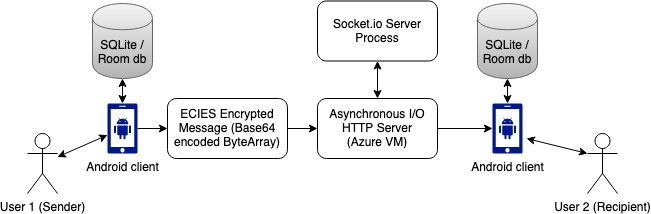
\includegraphics[scale=0.5]{images/high-level-architecture.png}
\caption{High level architecture of the system}
\end{figure}

\section{WebSockets vs REST API}
One of the major decisions required for this project was which transport protocol to use for propagating messages through the system. The two major options considered were REST APIs\cite{masse2011rest} and WebSockets\cite{fette2011websocket}. 

REST (Representational State Transfer) is a set of design principles which allow us to develop web services which utilise a central server and is based on the twin concepts of request and response. A client will send a request to a server and receive a response based on the content of the request. REST APIs are heavily used across many industries and mostly (though not exclusively) use the HTTP protocol to communicate between client and server. The primary weakness of REST is that it is not optimal for circumstances where constant bi-directional communication is important between client and server. Indeed, the WebSocket Protocol Standards Track Document\cite{fette2011websocket} states the problem as such:

\begin{verbatim}
Historically, creating web applications that need 
bidirectional communication between a client and a server 
(e.g. instant messaging and gaming applications) has required 
an abuse of HTTP to poll the server for updates while
sending upstream notifications as distinct HTTP calls.
\end{verbatim}

The WebSocket protocol is a newer system which excels in two-way communication between client and server systems. For chat applications like the subject of this project, WebSocket appears perfectly suited to the problem.  
Due to the comparative simplicity of bidirectional communication using WebSockets, the protocol uses significantly less energy\cite{herwig2015assessment} to maintain a client/server connection. This is especially relevant when considering that this is a mobile application which needs to preserve battery life. 

During the literature review of this topic, it became apparent that there was a way to achieve the best of both worlds. Socket.io\cite{rai2013socket} is a cross-platform library which initially attempts to create a WebSocket connection and, if not possible, falls back to HTTP polling. It also provides helpful additional features like automatic reconnection. It was determined that both client and server implementations existed in the desired languages (Python/Kotlin) and subsequently included in the system design.

The figure below describes the entire journey of a message through the messaging system. The colour scheme for the various key stages is broadly represented by the following:
\begin{enumerate}
	\item Green: Initial message composition, server querying and local storage.
	\item Yellow: Asymmetric + symmetric encryption, encoding and send process
	\item Red: Server routing for message
	\item Purple: Receipt, decryption, display and storage of message.
\end{enumerate}

\begin{figure}[H]
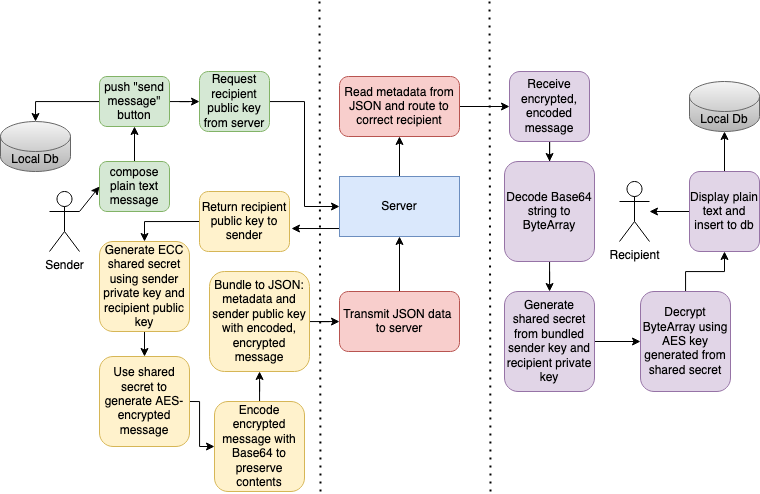
\includegraphics[scale=0.5]{images/message-flow.png}
\caption{Flowchart with high level view of entire lifecycle of a message}
\end{figure}

\section{Encryption Implementation}\label{encryption}
As mentioned previously, the system was designed with the prevailing goal of having two clients who could communicate with each other through an insecure, untrusted environment (i.e. the server) without needing to worry about message being vulnerable to man-in-the-middle attacks\cite{mallik2019man}.

Two of the most prevalent encryption approaches used in the modern world are asymmetric and symmetric encryption. Symmetric encryption is the simpler of the two options - a secret key is used to alter the content of a piece of plain text in such a way that it's unreadable to anyone except someone who also has the secret key and can use it to decrypt the message.

\cite{martinez2010comparison}Here is a placeholder for a piece of text about ECIES.
\subsection{Asymmetric component}\label{asymmetric}

\subsection{Symmetric component}\label{symmetric}

\subsection{Difficulties}\label{encryptionDifficulties}

\subsection{Storage of encryption keypair}

\section{Design Patterns}

\subsection{Dependency injection}

\subsection{Command pattern}

\subsection{Singleton pattern}

\subsection{Observer pattern}

\subsection{Adapter pattern}

\subsection{Data Access Object pattern}

\section{Persistence and storage considerations}
\subsection{Storage of self-destruct duration}
\subsection{Existing user persistence and reconnection flow}


\section{Development tooling}
There are two primary components to the overall system - one or more Android mobile client applications which communicate with a central, deployed server.


\subsection{Client}
The final client application was written entirely in Kotlin (v1.6.10) using the Android Studio IDE. 

\subsubsection{Development and debugging process}
Traditional Android software development involves using the qEmu device emulator built into Android Studio to imitate the experience of a real user on their own device. 

Debugging code during the HushChat development process was a complex endeavour, as the development machine had fairly limited RAM. As the purpose of the application was communication between two clients, it was important to be able to emulate two devices at the same time so messages could be exchanged. This was initially possible on the development machine, but became unfeasible over time as the complexity of the system grew and memory capacity became strained. 

The debugging environment eventually morphed into a single qEmu emulated device on the development machine combined with a physical android device (Google Pixel 4). This methodology became possible with the introduction of Android version 11 and Android Studio 'Bumblebee' (v2021.1), which allows the developer to run Android debugging tools (i.e the Android Debug Bridge, or ADB) wirelessly. This feature was extremely helpful in the development process, and it allowed for the introduction of further feature complexity that would not have been possible otherwise due to the technical limitations of the development machine. 

Running a WebSocket-based application locally also presented a minor challenge, as qEmu virtual devices use the traditional localhost/127.0.0.1 address to represent their own internal loopback interface rather than that of the host development machine. This meant that to communicate with the locally hosted server, the \href{https://developer.android.com/studio/run/emulator-networking.html}{special debugging address 10.0.2.2 was used.} After the development of the server side of the application was complete, this problem was solved by deploying the server to a static IP address (via a Azure Virtual Machine).


\subsubsection{Key Dependencies}
\begin{itemize}
	\item \href{https://github.com/socketio/socket.io-client-java}{Socket.io} - v2.0.0 - the developers of socket.io provide a native Java implementation. Due to Java's seamless interoperability with Kotlin, this did not cause any implementation problems with the version implemented.
	\item \href{https://www.bouncycastle.org/}{BouncyCastle} - v1.67 - BouncyCastle is the cryptography API that performs a lot of the cryptographic operations within the application, including generation of elliptic curve keypairs. There is a built-in version of BouncyCastle within the Android SDK, but this does not support ECC, which meant that the client application needed to replace the inbuilt library with a more updated version. This can be seen within the codebase with the following calls within the MainActivity and ChatWindow classes:
		\begin{verbatim}
		Security.removeProvider("BC")
		Security.addProvider(BouncyCastleProvider())
		\end{verbatim}
	\item \href{https://github.com/furnivall/SEng_Final_Project}{Room ORM} - v2.4.0 - Room provides an object-relational mapping (ORM) over the SQLite database built into the Android SDK. When developing the application, the main data model to consider on the client side was that of an individual chat message, including metadata (e.g. recipient) and content. Working with Room allowed for a more streamlined development experience and reduction of boilerplate code, as it meant working directly with Kotlin (Java) entities instead of writing complex queries for inserting messages to our viewmodel. SQL queries were still used to capture relevant data to display to the user in chat windows. 

\end{itemize}

\subsection{Server}
The server application was written in Python v3.9.1 in the PyCharm IDE and utilised several libraries which are highlighted below. 

\subsubsection{Key Dependencies}
\begin{itemize}
	\item \href{https://python-socketio.readthedocs.io/en/latest/index.html}{python-socketio} - v5.5.0 - a Python server implementation of socket.io, funded by the original socket.io developers.
	\item \href{https://docs.aiohttp.org/en/stable/}{aiohttp} - v3.8.1 - an asynchronous http server which (importantly) supports websockets. The socket.io process attaches itself to the aiohttp server which allows information to be transmitted and received from clients.
\end{itemize}

\subsubsection{Deployment}
To allow users to message other users, it was necessary to deploy the server application on a static IP. To do this, a 1GB/1CPU Virtual Machine instance was used, running Ubuntu 20.04 in the West Europe region of Microsoft Azure. 

\subsection{Final report}
This dissertation was written entirely in LaTeX using Neovim v0.5.1 with the VimTex plugin. 

\subsection{Version Control}
Git was the version control solution used throughout the project. Mild discomfort with the idea of storing the written report with a private company (Overleaf) while writing meant that it was worth taking the step of compiling the document locally. This had the fortunate benefit of meaning the entire project could be stored in a single git repository (as well as an opportunity to learn a lot of new things). 

The host of choice for the upstream repository on this project was GitHub, and the entirety of the project can be found at the following link: 

\begin{center}
\href{https://github.com/furnivall/SEng_Final_Project}{https://github.com/furnivall/SEng\_Final\_Project}
\end{center}

%%%%%%%%%%%%%%%%%%%%%%%%%%%%%%%%%%%%%%%%%%%%%%%%%%%%%%%%%%%%%%%%%%%
\chapter{Evaluation \& Testing}\label{testing}

%%%%%%%%%%%%%%%%%%%%%%%%%%%%%%%%%%%%%%%%%%%%%%%%%%%%%%%%%%%%%%%%%%%
\chapter{Conclusion}\label{conclusion}

\appendix % first appendix
%%%%%%%%%%%%%%%%%%%%%%%%%%%%%%%%%%%%%%%%%%%%%%%%%%%%%%%%%%%%%%%%%%%
\chapter{First appendix}

\section{Section of first appendix}

%%%%%%%%%%%%%%%%%%%%%%%%%%%%%%%%%%%%%%%%%%%%%%%%%%%%%%%%%%%%%%%%%%%
\chapter{Second appendix}

%%%%%%%%%%%%%%%%%%%%%%%%%%%%%%%%%%%%%%%%%%%%%%%%%%%%%%%%%%%%%%%%%%%
% it is fine to change the bibliography style if you want
\printbibliography
\end{document}
